% Chapter 2

\chapter{Cross-correlation} % Main chapter title

\label{Chapter2} % For referencing the chapter elsewhere, use \ref{Chapter2} 

\lhead{Chapter 3. \emph{Cross-correlation}} % This is for the header on each page - perhaps a shortened title

%----------------------------------------------------------------------------------------

%----------------------------------------------------------------------------------------
\section{The correlator}
\label{sec:about2}
\begin{figure}[htbp]
\center
    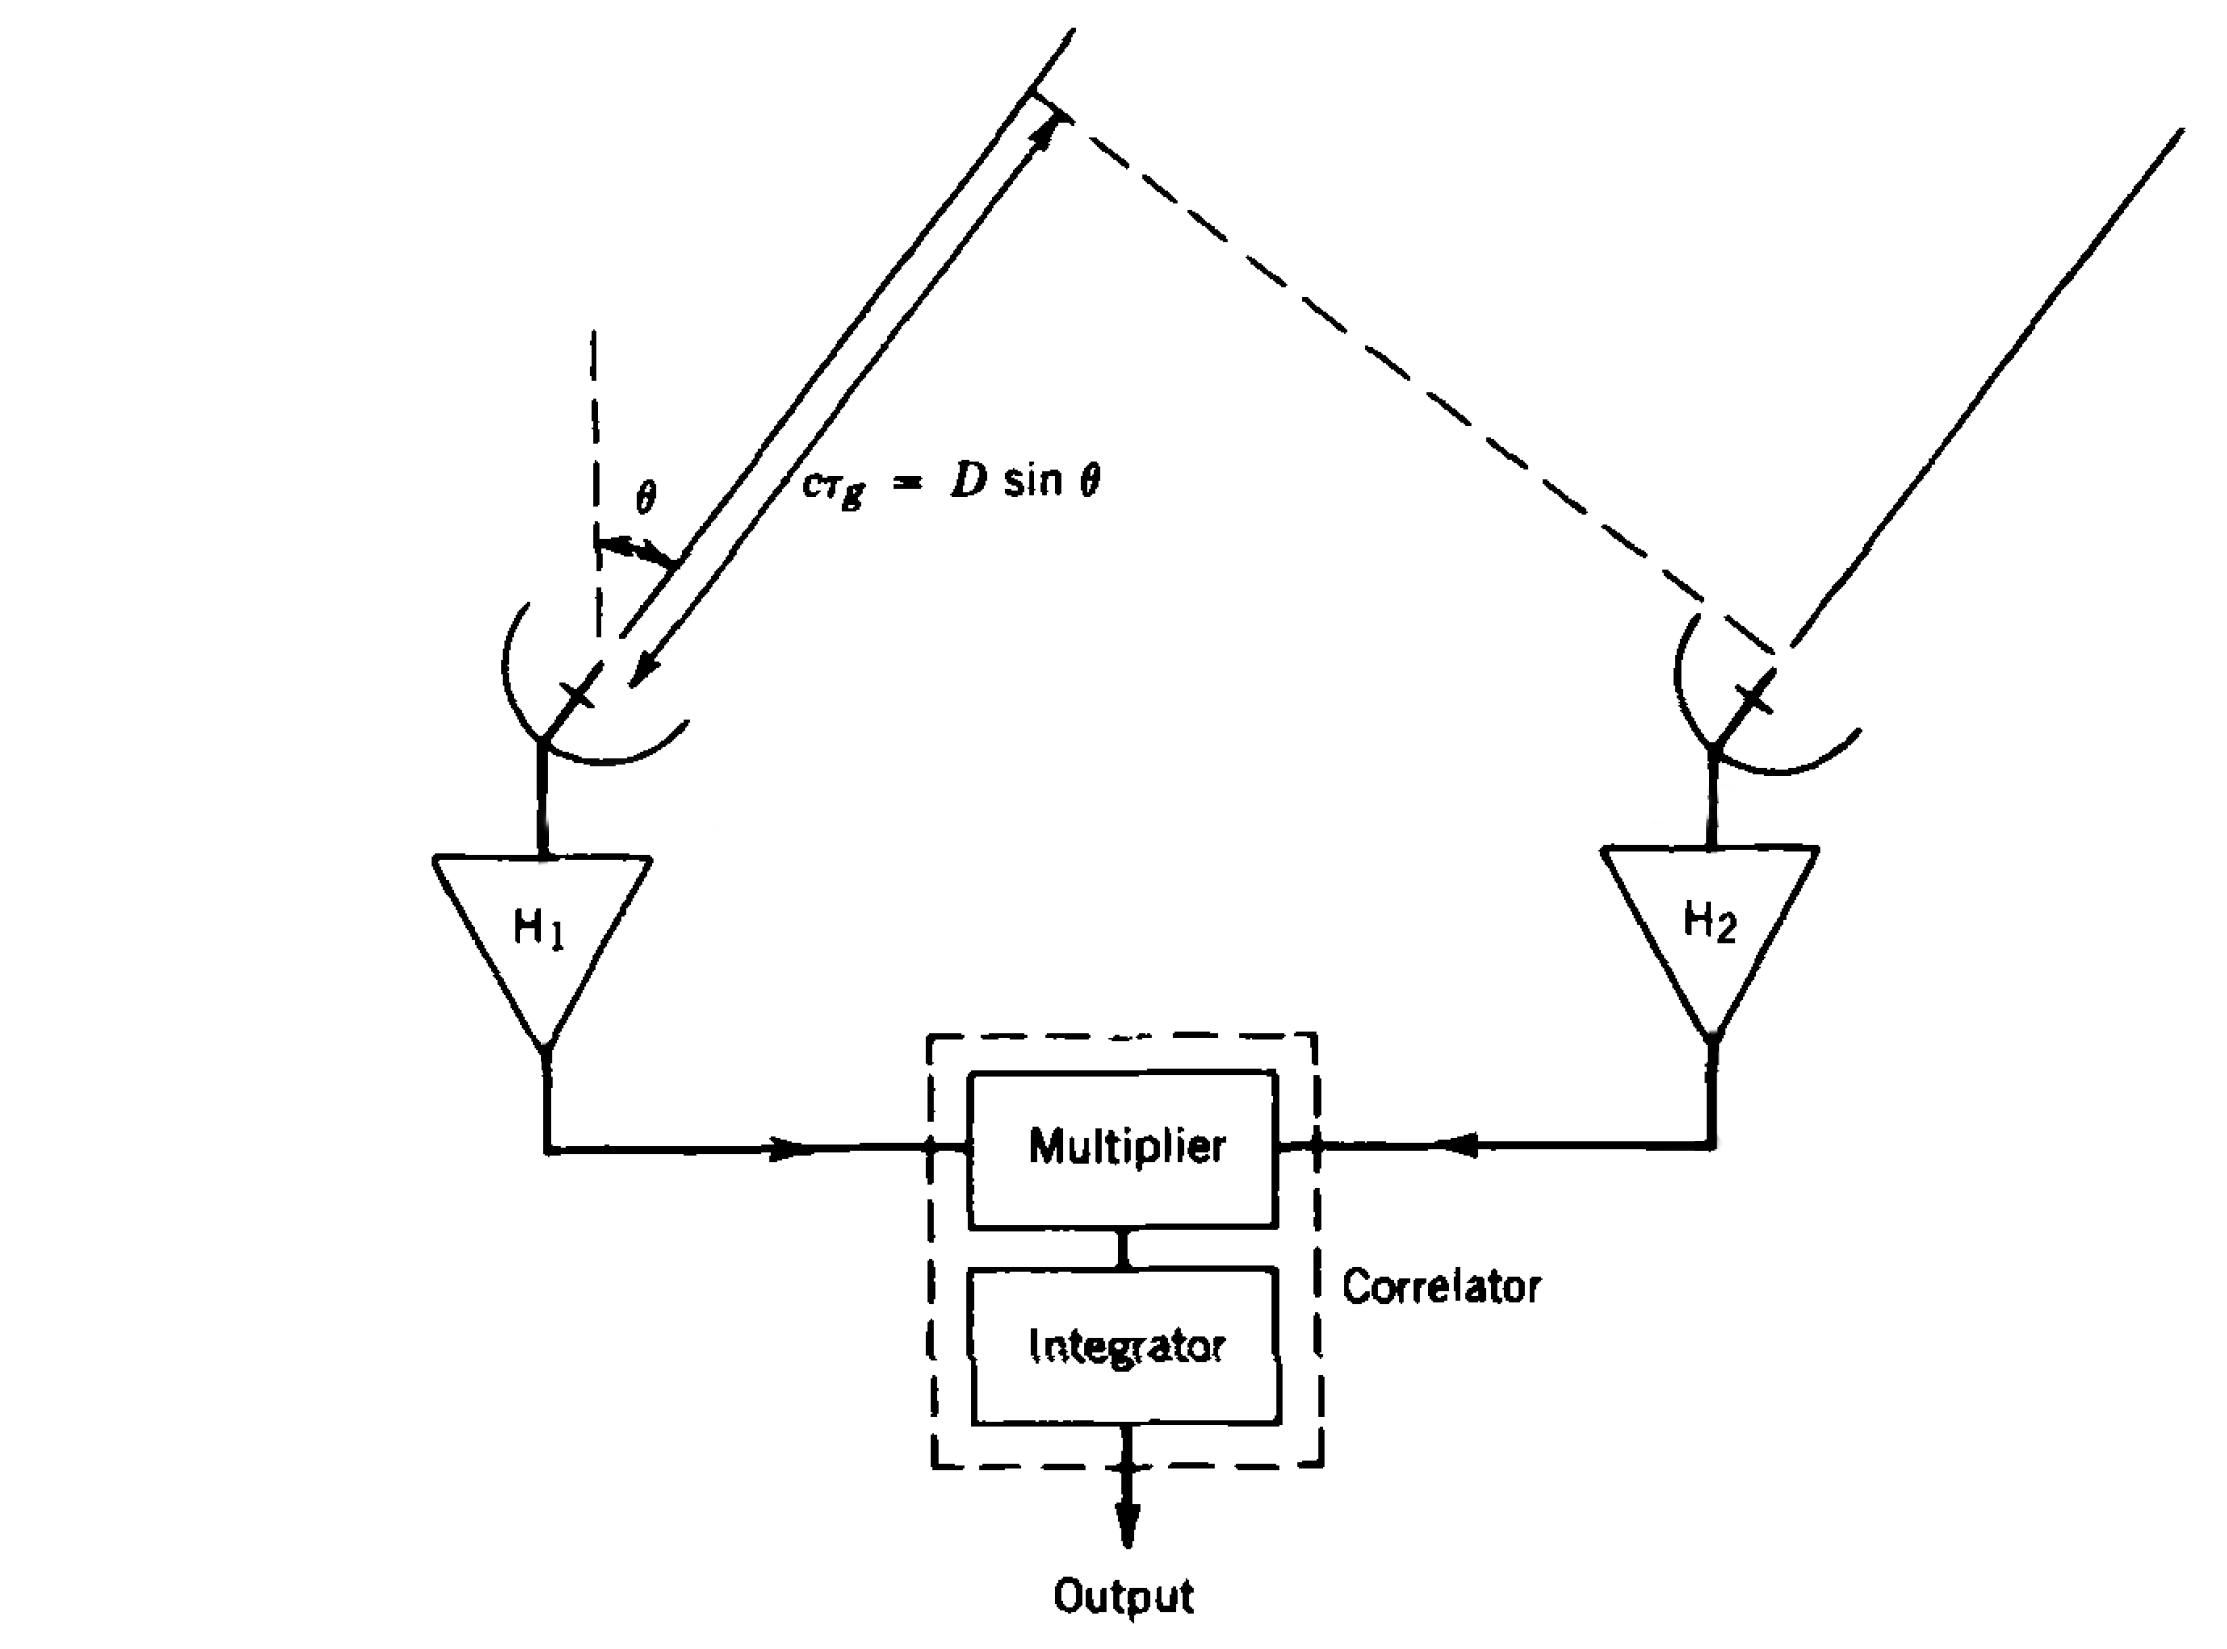
\includegraphics[scale= 0.15]{Figures/correlatorFil}
 	\caption[A simplistic representation of a correlator]{\\A simplistic representation of a correlator~\citep[Pg.~53,~Fig.~2.3]{thompson2008interferometry}}
	\label{fig:CorrelSet}
\end{figure}
{\citep[From][Sec~2.2]{thompson2008interferometry}}~One might ask, how do we get the values of visibilities? Remember that in chapter~\ref{Chapter1}, section~\ref{sec:intPrincipia}, last paragraph we said that it is a measure that characterises the relationship between the antenna-pair signal. Basically to obtain this measure, the antenna-pair signals is fed to a device which processes the inputs and outputs a signal which relates the input signals, there exist different types of devices that one might use to obtain that information, i.e., the visibility, in our case we will focus on the use of a correlator.\\
Basically a correlator does the following things as illustrated in figure~\ref{fig:CorrelSet} it multiplies the signals together and integrates over a certain interval of time called the integration time. Now assume that for a point source each antenna delivers the same signal, i.e. the voltage, $V(t)$, to the correlator and that one lags the other by a time delay, $\tau$, the output of the correlator may be a voltage, a current, or a coded set of logic levels (for a digital system), but in any case it represents a physical quantity with the dimensions of voltage squared. And we can express it as in the following equation~\ref{eq:correlOut},
\begin{equation}
\label{eq:correlOut}
r(\tau) = \lim_{T \to \infty}\frac{1}{2T}\int^{T}_{-T}{V(t)V(t-\tau)dt}
\end{equation}
This is actually an autocorrelation function.
%%
%Refine the following please include filter in the corelator image
%%
The signal from a natural cosmic source can be considered as a continuous random process that results in a broad spectrum, of which the phases are a random function of frequency. Assume that the time-averaged amplitude of the cosmic signal in any finite band is constant with frequency over the passband of the receiver. The squared amplitude of a frequency spectrum is known as the power density spectrum, or power spectrum. The power spectrum of a signal is the Fourier transform of the autocorrelation function of that signal. This statement is known as the Wiener-Khinchin relation which can be written as the following,
\begin{equation}
\label{eq:WKRelPow}
|H(\nu)|^2 = \int^{\infty}_{-\infty}{r(\tau)e^{-j2\pi{\nu{\tau}}} d\tau}
\end{equation} 
and its pair,
\begin{equation}
\label{eq:WKRelAut}
 r(\tau) = \int^{\infty}_{-\infty}{|H(\nu)|^2{e^{j2\pi{\nu{\tau}}}} d\nu}
\end{equation} 
\section{Cross-correlation}
\label{sec:crxcorrelabt}
{\citep[From][Sec.~3.3]{thompson2008interferometry}}~It is also useful to examine the corresponding relation for the \textbf{cross-correlation function} of two different waveforms. The response of a correlator, as used in a radio interferometer, can thus be written as

\begin{equation}
\label{eq:CrxOut}
r(\tau) = \lim_{T \to \infty}\frac{1}{2T}\int^{T}_{-T}{V_1(t){V_2}^{*}(t-\tau)dt}
\end{equation}
for which we have the pentagram as a short hand notation, as follows,
\begin{equation}
V_1(t)\star{V_2(t)} = \lim_{T \to \infty}\frac{1}{2T}\int^{T}_{-T}{V_1(t){V_2}^{*}(t-\tau)dt}
\end{equation}
From the convolution theorem one can very easily derive the following relationship,
\begin{equation}
V_1(t)\star{V_2(t)} \rightleftharpoons {\widehat{V}_1(\nu)\cdot{\widehat{V}^{*}_2(\nu)}}
\end{equation}
Where in all the previous and following equations the superscript asterisk{ }$^*$ denotes complex conjugation and, $\rightleftharpoons$, denotes Fourier transform.

Now let's get back to equation~\ref{eq:CrxOut}, $\tau$, is the time by which voltage $V_2$ is delayed with respect to voltage $V_1$. The functions $V_1$, and $V_2$ that represent the signals in equation~\ref{eq:CrxOut} may be complex. The output of a single multiplying device is a real voltage or number though. To obtain the complex cross-correlation, which represents both the amplitude and the phase of the visibility, one can record the fringe oscillations and measure their phase, or use a complex correlator which contains two multiplying circuits.\\

For the case where the antennas track the source, both the antenna beam center and the center of the source are at the $(l, m)$ origin, the correlator output can thus also be expressed as the following,
\begin{equation}
\label{eq:CrxSky}
r(\tau) = \int^{\infty}_{-\infty}\int^{\infty}_{-\infty}\int^{\infty}_{-\infty}{I(l,m)A(l,m){|H(\nu)|^2}e^{j2\pi{\nu}{\tau}}dldmd\nu}
\end{equation}

For a wavefront incident from the direction $(l, m)$, the difference in propagation times through the two antennas to the correlator results from a difference in path lengths of $(ul + vm)$ wavelengths, where an approximation has been made~(refer to the statement before and after Eq.~\ref{eq:Approx}). The corresponding time difference is $\frac{(ul + vm)}{\nu}$.
If we take as $V_1$, the signal from the antenna for which the path length is the greater (for positive $l$ and $m$), then from equation~\ref{eq:CrxSky}, the correlator output becomes
\begin{equation}
\label{eq:CrxSkylm}
r(\tau) = \int^{\infty}_{-\infty}\int^{\infty}_{-\infty}\int^{\infty}_{-\infty}{I(l,m)A(l,m){|H(\nu)|^2}e^{-j2\pi(lu + mv)}dldmd\nu}
\end{equation}

Assuming that the intensity and the antenna pattern are constant over the bandpass range of the filters, and the width of the source is small compared with the antenna beam. The correlator output then becomes 

\begin{eqnarray}
\label{eq:VisOut0}
r&=&\int^{\infty}_{-\infty}\int^{\infty}_{-\infty}{I(l,m)A(l,m)}dldm\int^{\infty}_{-\infty}{|H(\nu)|^2}e^{-j2\pi(lu + mv)}d\nu \\
&=& A_0{V(u,v)}\int^{\infty}_{-\infty}{|H(\nu)|^2}e^{-j2\pi(lu + mv)}d\nu  \label{eq:VisOut} 
\end{eqnarray}
where $A_0$ is the collecting area of the antennas in the direction of the maximum beam response and $V(u,v)$ the true visibility, the measured visibility, $V'(u,v)$ was introduced in chapter~\ref{Chapter1} in the equation~\ref{eq:visEq}. The filter response $H(\nu)$ is a dimensionless (gain) quantity, note that we assume that the antennas are identical and that their filter response are identical such that $H_1(\nu)=H_2(\nu)=H(\nu)$. If the filter response is essentially constant over a bandwidth, $A_0$, eq.~\ref{eq:VisOut} becomes
\begin{equation}
 r = A_0{V(u, v)}\Delta{\nu} 
\end{equation}
Thus we have here the visibility $V(u, v)$ which has units of Wm$^2$Hz$^{-1}$, $A_0$ has units of $m^2$, and $\Delta{\nu}$ has units of Hz. This is consistent with $r$, the output of the correlator, which is proportional to the correlated component of the received power. 
